\section{Experimentelles Vorgehen}

\subsection{Reversionspenel}
In diesem Versuch wird ein Pendel mit zwei Drehachsen und zwei Gewichten verwendet (siehe Abbildung \ref{fig:reversion}). Das eine Gewicht ist verstellbar. Dieses verstellbare Gewicht wird nun Stück für Stück um einen gewissen Abstand verschoben und die Schwingungsdauern von beiden Achsen gemessen. Hierfür wird eine Lichtschranke benutzt, um die Genauigkeit der Messung zu erhöhen. Es wird versucht zwei Punkte für das Gewicht zu finden, für den die Schwingungsdauern für beide Achsen gleich sind. Dies geschieht später über Interpolation der Daten. Hat man diesen Punkt gefunden, besitzt man die Schwingungsdauer des Reversionspendels und kann somit mit Formel \ref{eq:gravity} die Gravitation bestimmen, sofern der Abstand zwischen den Achsen (reduzierte Pendellänge) bekannt ist. Dieser wird mit einem Meterstab gemessen.

\begin{figure}
\centering
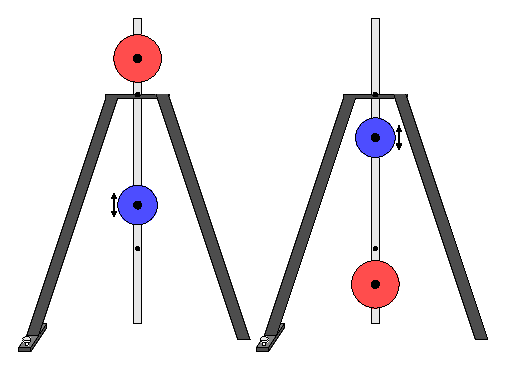
\includegraphics[width=0.5\textwidth]{Bilder/Versuch1.eps}
\caption{Aufbau des Reversionspendels mit zwei Achsen und einem beweglichen Gewicht (blau)}
\label{fig:reversion}
\end{figure}


\subsection{Gekoppelte Pendel}
Für den Versuch mit gekoppelten Pendeln werden zwei gleiche Pendel (gleiches Drehmoment, gleiche Schwingungsdauer, siehe Abbildung \ref{fig:gekoppelt}) verwendet. Zu Beginn wird die Schwingungsdauer der Pendel ohne Feder gemessen, anschließend werden zwei verschiedene Federn in jeweils vier Positionen eingehängt und die Auslenkung mit dem Computer für Schwingungen der Pendel in Phase, in Gegenphase und für eine Schwebung (nur ein Pendel wird ausgelenkt) gemessen. Für die zweite Feder wird aus Zeitgründen nur für eine Position der Feder gemessen.

\begin{figure}
\centering
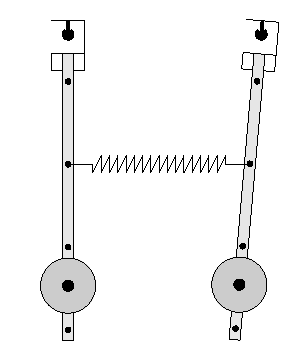
\includegraphics[width=0.3\textwidth]{Bilder/Versuch2.eps}
\caption{Aufbau der gekoppelten Pendel mit Feder und vier Löchern zum Einhängen der Federn}
\label{fig:gekoppelt}
\end{figure}